\documentclass[9pt,aspectratio=169]{beamer}

\usetheme{graham}

\title{Probability}
\subtitle[Graham Middle School]{Graham Middle School Math Olympiad Team}

\begin{document}

\maketitle

\begin{frame}{Probability}
  \begin{columns}[T]
    \begin{column}{0.5\textwidth}
      \begin{definition}
        An \textbf{outcome} is a possible result of an experiment.
      \end{definition}

      \begin{wrapfigure}[5]{r}{0.25\textwidth}%
        \vspace{-1em}
        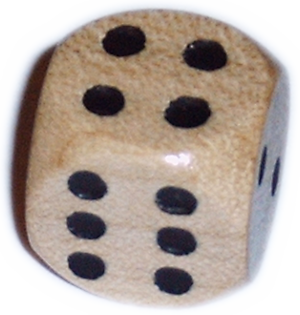
\includegraphics[width=0.25\textwidth]{03 - Probability/dice-4.png}
      \end{wrapfigure}
      We say "the outcome of throwing the dice was $4$." The experiment was throwing the die and its result (outcome) was that the face with $4$ pips on it came up.\medskip
  
      \begin{problem}
        We write each of the names of all $30$ students in a math club on a card and we draw a card at random. If there are $14$ sixth-graders, $9$ seventh-graders, and $7$ eighth-graders in this club, what is the probability of the name on the card being that of a sixth-grader? 
      \end{problem}
      The total number of \emph{outcomes} is all students in the club. The desired \emph{outcomes} are all sixth-graders. So \emph{probability} is
      \[
        P = \frac{14}{30} = \frac{7}{15}.
      \]
    \end{column}
    \begin{column}{0.5\textwidth}
      \begin{definition}
        If the number of outcomes is countable and \emph{if all outcomes have the same probability}, then \mbox{the~\textbf{probability}} of desired outcome is:
        \[ P = \frac{\text{(number of desired outcomes)}}{\text{(total number of events)}}. \]
        \vspace*{-1.5ex}
      \end{definition}

      Probability problems are either based on \emph{countable} outcomes or on outcomes that are not countable. The later case is called \emph{geometric probability} or \emph{continuous probability}.

      \begin{definition}
        In the \emph{geometric case}, the \textbf{probability} of a desired outcome is calculated as the ratio:
        \[ P = \frac{\text{(desired area)}}{\text{(total area)}}. \]
        \vspace*{-1.5ex}
      \end{definition}

      Probabilities in any case are always between $0$ and $1$, inclusive.

      Probability is sometimes also given in percent:
      \[ 𝑃(\text{in percent}) = 𝑃(\text{as a decimal or fraction}) \times 100\%. \]

    \end{column}
  \end{columns}
\end{frame}

\begin{frame}{Addition rule for probability}
  \begin{columns}[T]
    \begin{column}{0.5\textwidth}
      \begin{problem}
        What is the probability of choosing \emph{an ace} \textbf{or} \emph{a king} from a full deck of $52$ cards?
      \end{problem}
      \begin{wrapfigure}[6]{r}{0.20\textwidth}%
        \vspace{-1em}
        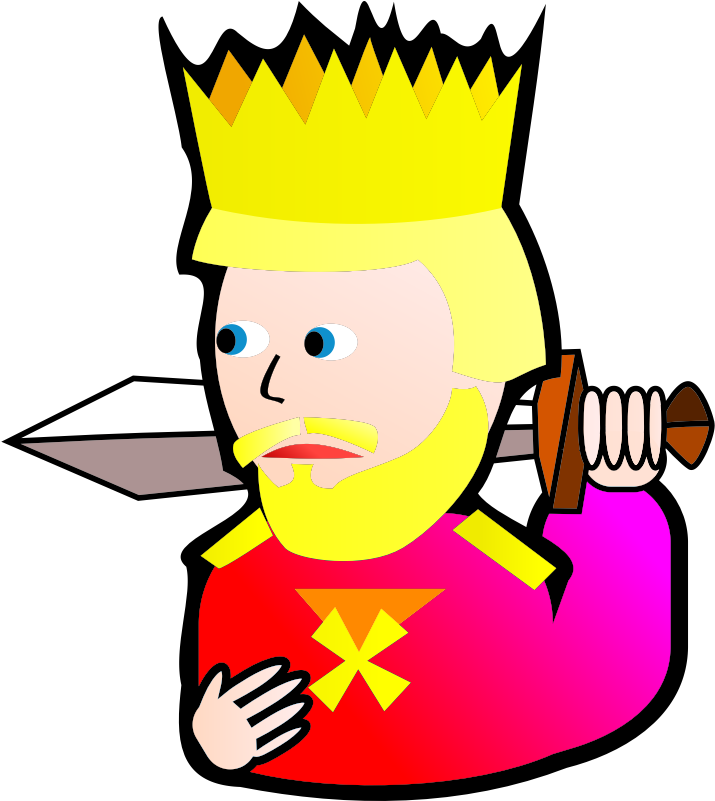
\includegraphics[width=0.25\textwidth]{03 - Probability/king-clip-art.png}
      \end{wrapfigure}
      \mbox{A card that we got from the deck of cards} may not be both an ace and a king. So we have $4$ \emph{outcomes} of getting an ace and $4$ \emph{outcomes} of getting a king. The result number of \emph{desired outcomes} is $8$. The \emph{total number of possible outcomes} is $52$.
      The total probability is
      \[ P = \frac{4 + 4}{52} = \frac{8}{52} = \frac{2}{13}. \]
      We also may count the probability in other way. The \emph{probability} of getting an ace is $4/52$ and the \emph{probability} of getting a king is also $4/52$. Since both cases are good for us, the total probability is
      \[ P = \frac{4}{52} + \frac{4}{52} = \frac{1}{13} + \frac{1}{13} = \frac{2}{13}. \]
    \end{column}
    \begin{column}{0.5\textwidth}
      \begin{definition}
        If two events are \emph{outcomes} of one experiment and they \emph{may not happen together}, then \emph{probability} of any of this event is \textbf{sum of their probabilities}
        \[ P(A\ \text{or}\ B) = P(A) + P(B). \]
        \vspace*{-2.5ex}          
      \end{definition}

      \begin{problem}
        What is the probability of choosing \emph{a multiple of $4$} or \emph{a multiple of $5$} from a numbers from $1$ to $100$?
      \end{problem}
      The probability of getting a multiple of $4$ is $25/100$, the probability of getting a multiple of $5$ is $20/100$. But there are multiples of $20$, which we counted twice. To make up for this case, we need to subtract the probability of getting a multiple of $20$, which is $5/100$. So total probability would be
      \[
        P = \frac{25}{100} + \frac{20}{100} - \frac{5}{100} = \frac{25 + 20 - 5}{100} = \frac{40}{100} = \frac{2}{5}.
      \]
      \begin{definition}
        So the \emph{probability of two events} of one experiment
        \[ P(A\ \text{or}\ B) = P(A) + P(B) - P(A\ \text{and}\ B). \]
        \vspace*{-2.5ex}          
      \end{definition}
    \end{column}
  \end{columns}
\end{frame}

\begin{frame}{Multiplication rule for probability}
  \begin{columns}[T]
    \begin{column}{0.5\textwidth}
      \begin{problem}
        If the experiment \emph{"throw a die and toss a coin"} is performed, what is the probability of the event \emph{"a~$4$~and a tails"} to happen?
      \end{problem}
      \begin{wrapfigure}[4]{l}{0.2\textwidth}%
        \vspace{-1.6em}
        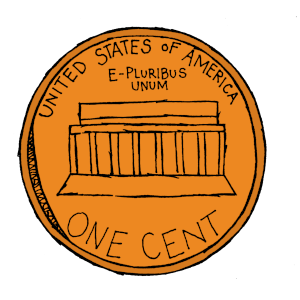
\includegraphics[width=0.23\textwidth]{03 - Probability/tail.png}
      \end{wrapfigure}
      Let's first throw a die. If $4$ didn’t happen, we don’t need to toss a coin, the desired event will not happen in any case. So we need to toss a~coin only when the die rolls~$4$. The $4$ has a probability of $1/6$ and, in this case only, we toss a coin and with a~probability of $1/2$ we will get tails. So the overall probability would be
      \[ P = \frac{1}{6} \cdot \frac{1}{2} = \frac{1}{12}. \] 

      \begin{definition}
        If two events are \emph{independent} the \textbf{probability} of both of them happen is \emph{a multiple of their probabilities}
        \[ P (A\ \text{and}\ B) = P (A) \cdot P (B). \] 
        \vspace*{-2ex} 
      \end{definition}
    \end{column}
    \begin{column}{0.5\textwidth}
      \begin{definition}
        The \textbf{conditional probability} of an event $E$ that depends on another event $F$ to happen is denoted 
        \[ P(E \mid F) \]
        and is probability of $E$ to happen if we know that $F$ has already happened.
      \end{definition}
      {\small We used that rule to solve the problem \emph{"throw a die and toss a coin"}.}
      \begin{definition}
        If two events are \emph{dependent} the \textbf{probability} of both of them happening is
        \[ P (A\ \text{and}\ B) = P (A) \cdot P (B \mid A). \] 
        \vspace*{-2.5ex} 
      \end{definition}
      {\small
        \begin{problem}
          What is the probability of choosing \emph{an ace} \textbf{and then} \emph{a~king} from a full deck of $52$ cards?
        \end{problem}
        The probability to choose an ace is $4/52$. Then we select a king from the deck without one card, so the probability to choose a king is $4/51$. The total probability~is
        \[ P(A \text{ and then } K) = P(A) \cdot P(K \mid A) = \frac{4}{52} \cdot \frac{4}{51} = \frac{4}{663}. \]
      }
    \end{column}
  \end{columns}
\end{frame}

\begin{frame}{Using the negative case}
  \begin{columns}[T]
    \begin{column}{0.5\textwidth}
      All possible outcomes of an experiment must equal the entire experiment.  That means that the probability for all outcomes is
      \[ P(\text{All outcomes}) = 1. \]
      \vspace*{-1em}
      \begin{problem}
        What is the probability if throwing the dice and not to get $4$. 
      \end{problem}
      There are $5$ outcomes that are desired: $1$, $2$, $3$, $5$, and $6$. So total probability would be 
      \[ P(\text{not throwing $4$}) = 5 \cdot \frac{1}{6} = \frac{5}{6}. \]
      On the other hand there is only one event that is not desired, so we can calculate the same probability as
      \begin{multline*} 
        P(\text{not throwing $4$}) = \\
        = P(\text{all possible results}) - P(\text{throwing $4$}) = \\
        = 1 - \frac{1}{6} = \frac{5}{6}.
      \end{multline*}
    \end{column}
    \begin{column}{0.5\textwidth}
      \begin{definition}
        The \textbf{complement event} of a \emph{desired event $E$}, denoted as $\overline{E}$, is the event that $E$ does not occur. Since for any event we know whether it is desired or not
        \[ P(\overline{E}) = 1 - P(E). \]
        \vspace*{-2.5ex} 
      \end{definition}
      Sometimes that simplifies the solution.
      \begin{problem}
        We are drawing $4$ cards from a full deck of cards. What is the probability to get \emph{at least one ace}?
      \end{problem}
      If we try to solve the problem using the \emph{conditional probability} we find out that number of cases is pretty big. But we may count the probability to \emph{not get any ace}.
      \[ P (\text{no ace}) = \frac{48}{52} \cdot \frac{47}{51} \cdot \frac{46}{50} \cdot \frac{45}{49} = \frac{38916}{54145} \approx 72\%.\]\\[-1ex]
      And probability to get \emph{an ace with $4$ cards} is
      \[ P (\text{at least one ace}) = 1 - \frac{38916}{54145} = \frac{15229}{54145} \approx 28 \%. \]
    \end{column}
  \end{columns}
\end{frame}

\begin{frame}{The birthday problem}
  \begin{columns}[T]
    \begin{column}{0.5\textwidth}
      \begin{problem}
        How many people need to attend a party until there is a $50\%$ chance that at least two guests share a birthday?
      \end{problem}
      It is easier to calculate the probability that \emph{no two people share a birthday}. 
      
      Les's start with the first guest. He doesn't share a birthday with anyone. So the probability is $1$.
      
      The second guest may share a birthday with the first guest with probability $364/365$. 
      
      The third one doesn't share a birthday with previous guests with probability $363/365$ and so on. 
      
      For $n$ guests
      \begin{multline*}
        P(\text{no shared birthday}) = \\
        = \frac{365}{365} \cdot \frac{364}{365} \cdot \frac{363}{365} \cdot \ldots \cdot \frac{365 - n + 1}{365} = \\ = \frac{365!}{(365-n)!} \cdot \frac{1}{365^n}.
      \end{multline*}
    \end{column}
    \begin{column}{0.5\textwidth}
      Using formula 
      \begin{multline*}
         P(\text{there is a shared birthday}) = \\ 
         = 1 - P(\text{no shared birthday})
      \end{multline*}
      we can calculate, using computer, the probability for any number of guests
      \begin{center}
        \vspace*{-1ex}   
        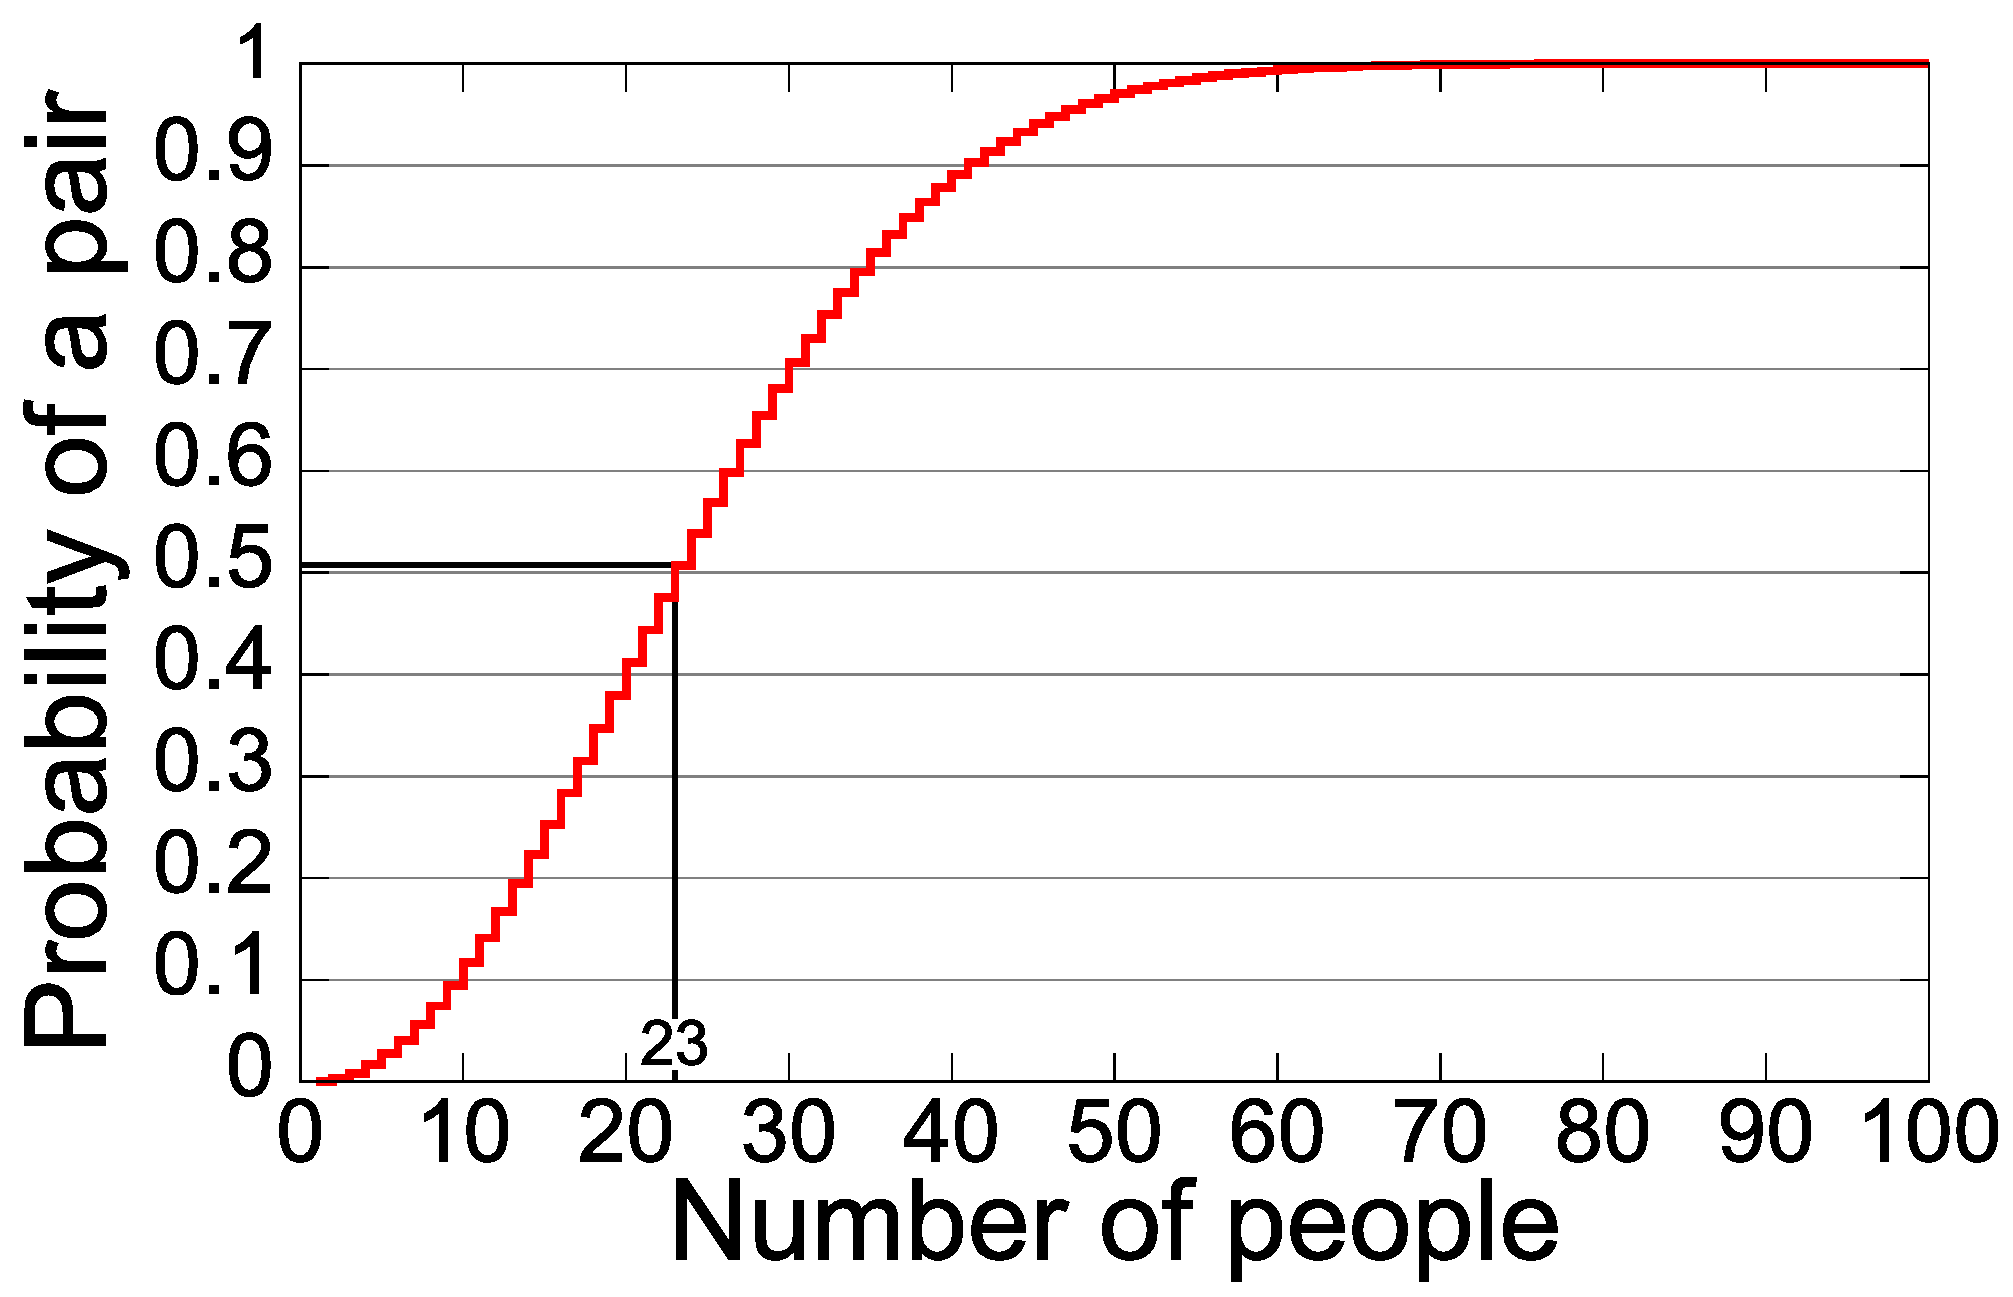
\includegraphics[width = 0.80\textwidth]{03 - Probability/Birthday_Paradox.pdf}
        \vspace*{-1ex}   
      \end{center} 
      So we may see that group of $23$ people has the probability of $50.7\%$ to have a shared birthday, and group of $70$ people has probability of $99.9\%$ to~share a birthday.
    \end{column}
  \end{columns}
\end{frame}

\begin{frame}{Sample problem 1}
  \begin{columns}[T]
    \begin{column}{0.5\textwidth}
      {\small
      \begin{problem}
        Mala and Joslyn number the cards in a deck of playing cards from $1$ to $52$. Mala and Joslyn each draw a card and show them to each other. What is the probability that the sum of the numbers on the cards is \emph{odd}? Express your answer as a common fraction.
      \end{problem}

      {\color{textBlue} Solution 1:} There are two ways for the sum to be \emph{odd}:  Mala draws an odd card and Joslyn draws an even, or vice versa.  If the both draw even or odd cards, the resulting sum is even.

      Using the \emph{addition rule for probability}, we add the probabilities from the two scenarios that lead to an odd sum.  Namely, 
      \[ P(\text{odd sum}) = P\left(\text{\parbox{5.3em}{Mala odd\\Joslyn even}}\right) + P\left(\text{\parbox{4.8em}{Mala even\\Joslyn odd}}\right). \]
      
      Now we use the \emph{product rule} to find the probabilities for each of those scenarios occurring.  Note that after Mala draws her card, there are only $51$ cards remaining in the deck, and $26$ of them are the opposite flavor of even/odd
      \[ P(\text{odd sum}) = \frac{1}{2} \cdot \frac{26}{51} + \frac{1}{2} \cdot \frac{26}{51} = \frac{26}{51}. \]
      }
    \end{column}
    \begin{column}{0.5\textwidth}
      {\small
      {\color{textBlue} Solution 2:} Use \emph{combinations}. The total number of ways to draw $2$ cards is $C_2^{52}$, which equals $\cfrac{52 \times 51}{2}$. The total number of combinations drawing $1$ even and $1$ odd is $\cfrac{52 \times 26}{2}$.  This is because we can select any card first, and then have $26$ cards remaining in the deck that make the sum odd.  We divide by $2$ because the order of drawing doesn’t matter in determining the number of combinations.\begin{multline*} 
        P(\text{odd sum}) = \\ = \frac{\text{Total ways to draw $1$ even and $1$ odd}}{\text{Total ways to draw $2$ cards}} = \\ = \frac{52 \times 26}{52 \times 51} = \frac{26}{51}
      \end{multline*}
      }
      \begin{example}
        The initial intuition is that probability should be $1/2$. But this is not a case, because once you draw the first card, the probabilities to draw odd/even card has changed.  
      \end{example}
    \end{column}
  \end{columns}
\end{frame}

\begin{frame}{Sample problem 2}
  \begin{columns}[T]
    \begin{column}{0.5\textwidth}
      \begin{problem}
        You have a bin containing $20$ \emph{red} socks and $40$ \emph{blue} socks.~You reach in and randomly pick out two socks. What is the probability, expressed as a~ratio~$a/b$, that you managed to pick out a matching pair (\emph{red/red} or \emph{blue/blue})?
      \end{problem}
      {\color{textBlue} Solution 1:} In this solution, we use the \emph{addition} and \emph{multiplication rules} for probability. Since there is no overlap between the \emph{red/red} and \emph{blue/blue} events, 
      {\small
      \[ P(\text{matching pair}) = P(\text{red/red}) + P(\text{blue/blue}).\] \vspace*{-1ex}}

      We use the \emph{multiplication rule} next, multiplying the probability of pulling out the sock of the first color by the probability of next pulling out a sock of the same color.
      {\small
      \[
        P(\text{red/red}) = \frac{20}{60} \cdot \frac{19}{59}, \qquad
        P(\text{blue/blue}) = \frac{40}{60} \cdot \frac{39}{59},
      \]
      \vspace*{-1ex}
      \begin{multline*}
        P(\text{matching pair}) = \\ = \frac{20 \times 19 + 40 \times 39}{60 \times 59} = \frac{19 + 78}{3 \times 59} = \frac{97}{177}.
      \end{multline*}
      }
    \end{column}
    \begin{column}{0.5\textwidth}
      {\color{textBlue} Solution 2:} 

      Use \emph{combinations}. There are $C_2^{20} = \frac{20 \times 19}{2}$ ways to pick $2$ \emph{red} socks out of $20$, and $C_2^{40} = \frac{40 \times 39}{2}$ ways to pick $2$ \emph{blue} socks out of $40$. The total number of ways to pick $2$ socks out of $60$ is $C_2^{60} = \frac{60 \times 59}{2}$.\vspace*{-1.5ex}
      {\small\[ P(\text{red/red}) = \frac{C_2^{20}}{C_2^{60}}, \qquad P(\text{blue/blue}) = \frac{C_2^{40}}{C_2^{60}}. \]}
      Since there is no overlap between \emph{red/red} and \emph{blue/blue} events, 
      {\small \[ P(\text{matching}) = \frac{20 \times 19 + 40 \times 39}{60 \times 59} = \frac{97}{177}. \]}
      \begin{wrapfigure}[5]{l}{0.35\textwidth}%
        \vspace{-2em}
        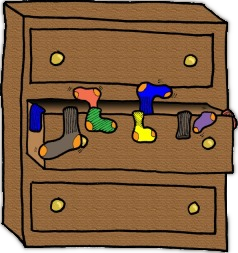
\includegraphics[width=0.35\textwidth]{03 - Probability/sock-drawer.png}
      \end{wrapfigure}
      
      Armed~with~your~knowledge of probability,~you~will~never be frightened of~sock~drawer problems again.
    \end{column}
  \end{columns}
\end{frame}

\begin{frame}{Exercises}
  \begin{columns}[T]
    \begin{column}{0.5\textwidth}
      \begin{enumerate}
        \item When a pair of $6$-sided dice are rolled, what is the probability that the numbers rolled sum to $7$?
        \item What is the probability of being dealt a $5$-card poker hand that is a royal flush (\emph{10-Jack- Queen-King-Ace}) of the same suit?
        \item In blackjack, you automatically win and get a larger payout if you are dealt two cards, one of which is an ace, and the other is a \emph{10, jack, queen, or king}.  What is the probability of being dealt such a two-card hand?
        \item With the score tied, a player who makes $50\%$ of her free throws is fouled while attempting a $3$-point shot at the buzzer, and earns $3$ free throws.  If she makes at least one shot, her team will win in regulation time.  What is the probability that she makes at least one of her free throws?
        \seti
      \end{enumerate}
    \end{column}
    \begin{column}{0.5\textwidth}
      \begin{enumerate}
        \conti
        \item If you flip a fair coin $5$ times, what is the probability that you will flip a total of $3$ heads and $2$ tails?
        \item I have $100$ marbles:  $20$ red, $40$ blue, $30$~green, $10$ black.  If I pick a marble, and then a second marble without replacing the first one, what is the probability that I will select a red marble and then a blue marble.
        \item If I start with the same $100$ marbles as in question {\color{darkOrange} 6}, and keep picking until no marbles remain, what is the probability that the last marble chose will be blue?
        \item If the missing digit $A$ in the number $579A6$ is chosen at random, what is the probability that the number is divisible by $3$?
      \end{enumerate}
    \end{column}
  \end{columns}
\end{frame}

\begin{frame}{Challenge problems}
  \begin{columns}[T]
    \begin{column}{0.5\textwidth}
      {\small
      \begin{enumerate}
        \item During the 2021 NBA playoffs, Giannis was a $50\%$ free throw shooter.  Bucking that trend, in the clinching game of the NBA finals, he made $17$ of his first $18$ free throws.  What is the probability that a $50\%$ shooter could accomplish this?  
        
        \emph{Note that this problem is equivalent to asking what is the probability of tossing heads $17$-of-$18$ times when flipping a fair coin.}
        \item On the TV show “Let’s Make a Deal,” there were $3$ doors.  Behind one door was a new car.  Behind the other two doors there were goats.  The contestant initially picks a door.  The host, Monte Hall, knows where the car is, and following the contestant’s guess, he always opens a door the contestant didn’t pick, and that doesn’t have the car behind it, revealing a goat, and leaving two doors unopened.  At this point, he asks the contestant if they want to keep their original guess, or switch to the other door. 
        
        What is the probability of winning the car if you switch? 
        What is the probability of winning if you keep your original guess? Should the contestant switch?
        \seti
      \end{enumerate}
      }
    \end{column}
    \begin{column}{0.5\textwidth}
      \begin{enumerate}
        \conti
        \item A 3-legged creature has an unorganized sock drawer with $4$ red socks, $6$ blue socks and $8$ yellow socks.
        \begin{center}
          \vspace*{-1ex}   
          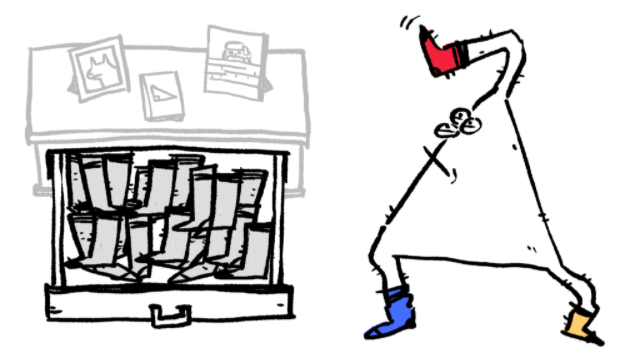
\includegraphics[width = 0.80\textwidth]{03 - Probability/3-leg-creature.png}
          \vspace*{-1ex}   
        \end{center} 
        The creature reaches into the sock drawer without looking and pulls out three random socks.  What is the probability that he pulls out a matching pair of $3$ socks?
      \end{enumerate}
    \end{column}
  \end{columns}
\end{frame}

% \begin{frame}{Team attack problems}
%   \begin{columns}[T]
%     \begin{column}{0.5\textwidth}
%       \begin{enumerate}
%         \item In one scenario in the board game risk, a~defender rolls a $6$-sided die, and the attacker rolls a pair of $6$-sided dice.  The higher attacking die is compared to the defending die, and the defender wins if its roll is greater than or equal to the higher attacking die.  What is the probability that the defender wins?
%         \item What is the probability that a positive integer less than $1000$ has units digit $4$ and is divisible by $7$?  Express your answer as a~common fraction.
        
%       \end{enumerate}
%     \end{column}
%     \begin{column}{0.5\textwidth}
%     \end{column}
%   \end{columns}
% \end{frame}

% \begin{frame}{Title}
%   \begin{columns}[T]
%     \begin{column}{0.5\textwidth}
%     \end{column}
%     \begin{column}{0.5\textwidth}
%     \end{column}
%   \end{columns}
% \end{frame}
\end{document}
